\section{Resultados}

As instâncias do problema do FlowShop utilizadas com a metaheurística ACO foram
as seguintes


\begin{figure}[htp]
  \begin{center}
    \subfigure[abz5]{\label{fig:edge-a}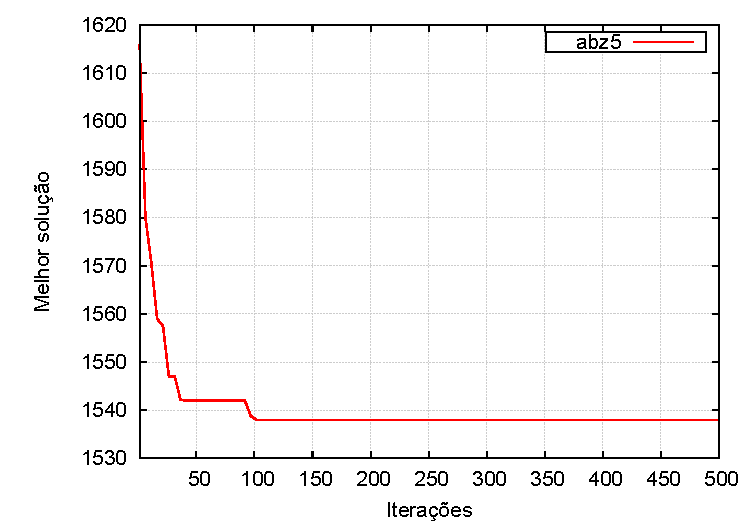
\includegraphics[scale=0.60]{fig/abz5.pdf}}
    \subfigure[car5]{\label{fig:edge-b}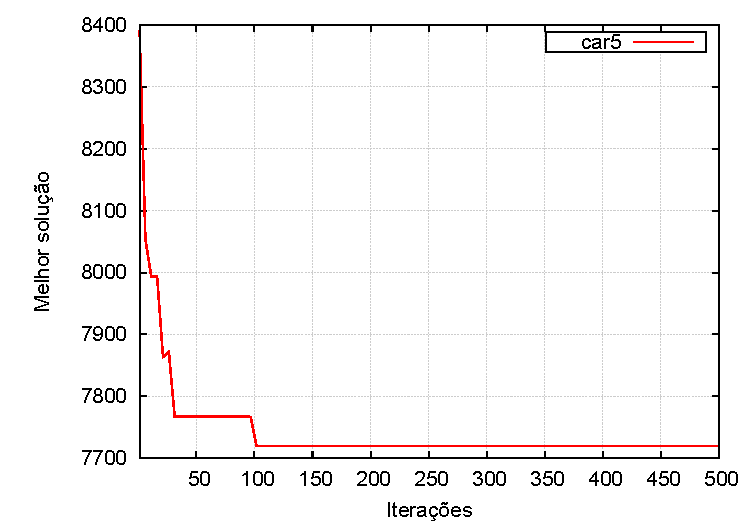
\includegraphics[scale=0.60]{fig/car5.pdf}}
    \\
  \end{center}
  \caption{Convergência do algoritmo Ant-System para as instâncias abz5 e car5}
  \label{fig:edge}
\end{figure}

	\begin{table}
	\centering
	\begin{tabular}{c|c|c|c||c||c|c|c||c}
	\hline\hline
	\multicolumn{4}{c||}{Instâncias Comparativas} & Solução 
	& \multicolumn{3}{|c||}{Solução Obtida} & Aproximação\\
	\hline
	Nº &  Referência & m & n & ``Ótima'' & Inicial & tempo (s) & Melhor & Gap\\
	\hline\hline
	1 & abz5 & 10 & 10 & 1544 & 1592 & 19.7 & 1538 & 0.99611399\\
	2 & car5 & 10 & 6 & 7720 & 8279 & 16.8 & 7720 & 1.0\\
	\hline\hline
	\multicolumn{8}{r||}{Média das aproximações com resultados conhecidos
	$\rightarrowtail$} & 0.998056995	\\
	\hline\hline
	Nº &  Referência & m & n & Inicial & Máxima & Média & Melhor & tempo (s)\\
	\hline\hline
	3 & hel11 & 100 & 10 & 569 & 555 & 552 & 549 & 5636.7 \\
	4 & rec07 & 20 & 10 & 1802 & 1670 & 1635 & 1582 & 51.76 \\
	5 & rec13 & 20 & 15 & 2268 & 2096 & 2052 & 1971 & 57.23 \\
	6 & rec37 & 75 & 20 & 5842 & 5786 & 5753 & 5713 & 2634.3 \\	
	7 & rec41 & 75 & 20 & 6037 & 5892 & 5835 & 5784 & 2656.9 \\
	\hline\hline
	\multicolumn{9}{c}{Instâncias Opcionais} \\
	\hline\hline
	Nº &  Referência & m & n & Inicial & Máxima & Média & Melhor & tempo (s)\\
	\hline\hline
	1 & car1 & 11 & 5 & 7835 & 7038 & 7038 & 7038 & 20.8 \\
	2 & car2 & 13 & 4 & 8148 & 7376 & 7292 & 7166 & 30.4 \\
	3 & car3 & 12 & 5 & 7731 & 7543 & 7425 & 7312 & 26.1 \\
	4 & car4 & 14 & 4 & 8841 & 8423 & 8085 & 8003 & 37.7 \\
	5 & car6 & 8 & 9 & 9588 & 8754 & 8608 & 8505 & 11.3 \\
	6 & car7 & 7 & 7 & 7181 & 6643 & 6621 & 6590 & 7.8 \\
	7 & car8 & 8 & 8 & 9102 & 8564 & 8447 & 8366 & 10.8 \\
	8 & rec01 & 20 & 5 & 1472 & 1360 & 1338 & 1322 & 95.3 \\
	9 & rec03 & 20 & 5 & 1281 & 1188 & 1162 & 1133 & 95.4 \\
	10 & rec05 & 20 & 5 & 1366 & 1284 & 1276 & 1269 & 95.1 \\
	\hline\hline
	\end{tabular}
	\end{table}
